 \usetikzlibrary{arrows}
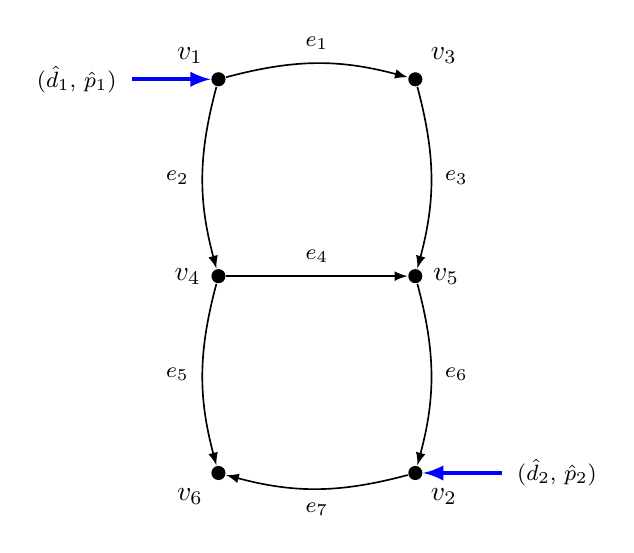
\begin{tikzpicture}[-latex ,auto,semithick,state/.style ={ draw,shape=circle,scale=1}]

\node[circle,fill,inner sep=1.8pt,label=above left: $v_1$] (A) at (0,0) {};
\node[circle,fill,inner sep=1.8pt,label=above right: $v_3$] (B) at (2.5,0) {};
\node[circle,fill,inner sep=1.8pt,label= left: $v_4$] (C) at (0,-2.5) {};
\node[circle,fill,inner sep=1.8pt,label= right: $v_5$] (D) at (2.5,-2.5) {};
\node[circle,fill,inner sep=1.8pt,label= below right: $v_2$] (E) at (2.5,-5) {};
\node[circle,fill,inner sep=1.8pt,label= below left: $v_6$] (F) at (0,-5) {};


\path (A) edge [bend right = -15] node[above  =0.05 cm] {\footnotesize$e_{1}$} (B);
\path (A) edge [bend right = 15] node[left  =0.05 cm] {\footnotesize$e_{2}$} (C);
\path (B) edge [bend right = -15] node[right  =0.05 cm] {\footnotesize$e_{3}$} (D);
\path (C) edge [bend right = 0] node[above  =0.05 cm] {\footnotesize$e_{4}$} (D);
\path (C) edge [bend right = 15] node[left  =0.05 cm] {\footnotesize$e_{5}$} (F);
\path (D) edge [bend right = -15] node[right  =0.05 cm] {\footnotesize$e_{6}$} (E);
\path (E) edge [bend right = -15] node[below  =0.05 cm] {\footnotesize$e_{7}$} (F);

\draw [-latex,line width=1.5pt,blue](-1.1,0) -- (-0.1,0);
\draw [-latex,line width=1.5pt,blue](3.6,-5) -- (2.6,-5);
\node at (-1.8,0) {\footnotesize $(\hat{d}_1$, $\hat{p}_1)$};
\node at (4.3,-5) {\footnotesize $(\hat{d}_2$, $\hat{p}_2)$};
\end{tikzpicture}
